\section{TRIỂN KHAI MÔ HÌNH HYBRID SEARCH}
\subsection{Tổng quan về Azure VM - Nền tảng máy ảo triển khai ứng dụng}
\hspace*{1cm}
Bước tiếp theo trong quá trình triển khai, ta cần thực hiện việc triển khai mô hình hybrid search. Do đây là mô hình khá nặng về dung lượng cũng như cần tài nguyên tính toán cao nên cần được triển khai trên một nền tảng độc lập tách biệt với nền tảng \textit{back-end}. Cách tiếp cận của nhóm khi triển khai mô hình này đó là thực hiện triển khai trên một máy ảo từ xa. Hiện nay, cả ba dịch vụ điện toán đám mây hàng đầu là \textit{Google Cloud}, \textit{Microsoft Azure} và \textit{Amazon Web Services} đều cung cấp dịch vụ cho thuê máy ảo, hỗ trợ tốt các hệ điều hành phổ biến hiện nay như \textit{Windows} hay \textit{Linux}. Sau khi đã xem xét và tìm hiểu, nhóm quyết định chọn triển khai với máy ảo với dịch vụ của \textit{Microsoft Azure}. Các lợi ích có thể kể đến mà máy ảo do \textit{Microsoft Azure} cung cấp đó là:
\begin{itemize}
    \item \textit{Tính linh hoạt và mở rộng:} \textit{Azure} cung cấp khả năng mở rộng linh hoạt, cho phép người sử dụng dễ dàng tăng hoặc giảm tài nguyên máy ảo theo nhu cầu kinh doanh. người sử dụng có thể thay đổi cấu hình máy ảo như \textit{CPU}, \textit{RAM}, và dung lượng lưu trữ một cách nhanh chóng.
    \item \textit{Chi phí hiệu quả:} \textit{Azure} cung cấp nhiều tùy chọn giá cả, bao gồm mô hình thanh toán theo mức sử dụng \textit{(pay-as-you-go)}, giúp người sử dụng chỉ phải trả tiền cho những gì người sử dụng sử dụng. Điều này giúp tiết kiệm chi phí và tránh lãng phí tài nguyên.
    \item \textit{Độ tin cậy và hiệu suất cao:} \textit{Azure} đảm bảo mức độ khả dụng cao với các cam kết \textit{SLA (Service Level Agreement)} lên đến 99.95\% cho các máy ảo, đảm bảo rằng ứng dụng và dịch vụ của người sử dụng luôn hoạt động ổn định và hiệu quả.
    \item \textit{Bảo mật mạnh mẽ:} \textit{Azure} tích hợp nhiều tính năng bảo mật như mã hóa dữ liệu, quản lý danh tính và truy cập \textit{(IAM)}, và các công cụ bảo vệ trước các mối đe dọa mạng. \textit{Azure Security Center} giúp người sử dụng theo dõi và quản lý bảo mật toàn diện.
\end{itemize}
\subsection{Thực hiện triển khai mô hình hybrid search trên máy ảo Azure VM}
\hspace*{1cm}
Để bắt đầu việc thực hiện triển khai mô hình trên nền tảng máy ảo \textit{Azure VM}, bước đầu tiên ta cần có tài khoản \textit{Microsoft}, để hưởng chính sách ưu đãi dành cho học sinh, sinh viên, ta có thể sử dụng địa chỉ \textit{email} do trường cung cấp để đăng ký. Ưu đãi đó bao gồm việc sử dụng đa dạng các dịch vụ miễn phí trong vòng một năm, ngoái ra tài khoản cũng sẽ được cung cấp sẵn \$100.0 để mua thêm các dịch vụ nâng cao để sử dụng. Sau khi đã có tài khoản \textit{Microsoft}, ta sẽ cần truy cập vào trang chủ của \textit{Microsoft Azure} và thực hiện bước đầu tiên là tạo ra một \textit{Resource Group}, đây được hiểu là một môi trưởng tài nguyên được triển khai một cách độc lập bao gồm các dịch vụ hoạt động bên trong môi trường này, và được triển khai ở một vùng nhất định trên thế giới, nơi có đặt trung tâm dữ liệu của \textit{Microsft}. Ở đây nhóm thực hiện tạo một \textit{Resource Group} với tên là \textit{ResourceGroup-Primary}, được triển khai ở máy chủ đặt tại \textit{Singapore}.
\begin{figure}[H]
    \centering
    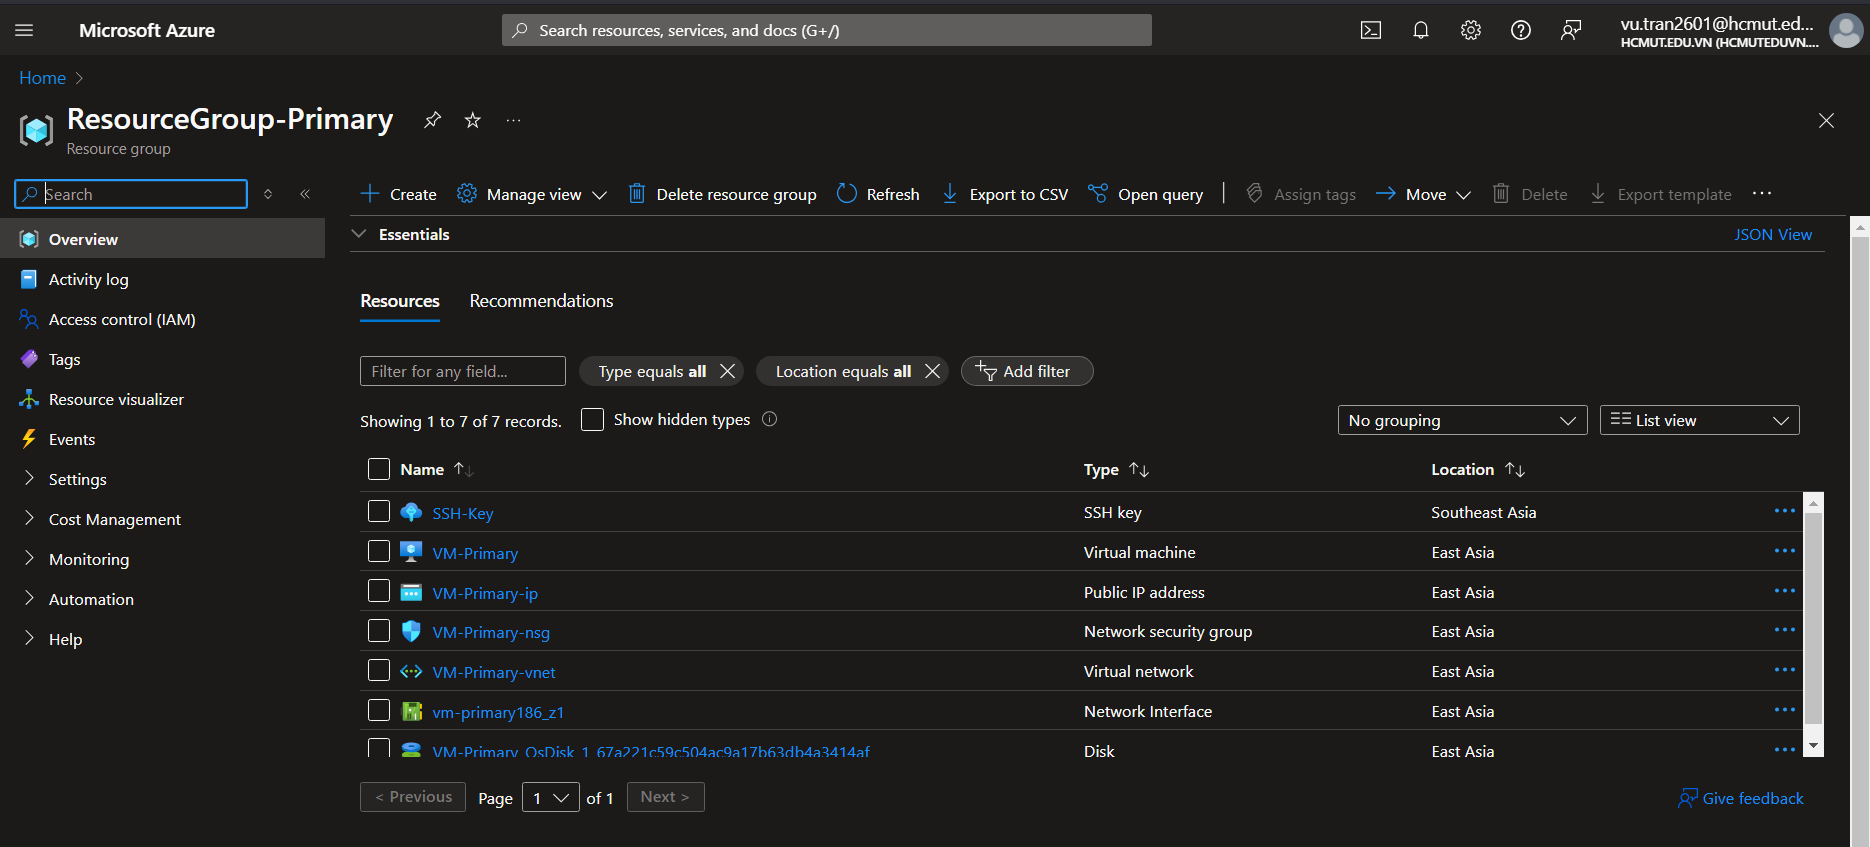
\includegraphics[width=1\textwidth]{Images/Deployment/HybridSearch/ResrouceGroup.png}
    \caption{Resource Group với tên là Resource Group được khởi tạo thành công}
\end{figure}
\hspace*{1cm}
Sau khi đã khởi tạo thành công \textit{Resource Group}, ta đã có thể tiến hành việc tạo ra một máy ảo để bắt đầu quá trình triển khai. Trước tiên ta trở vê trang chính của \textit{Microsoft Azure Portal} và chọn \textit{Virtual Machine}. Sau đó, trang chủ sẽ hiển thị giao diện để người dùng thực hiện các bước cấu hình cần thiết trước khi chạy máy ảo.
\begin{figure}[H]
    \centering
    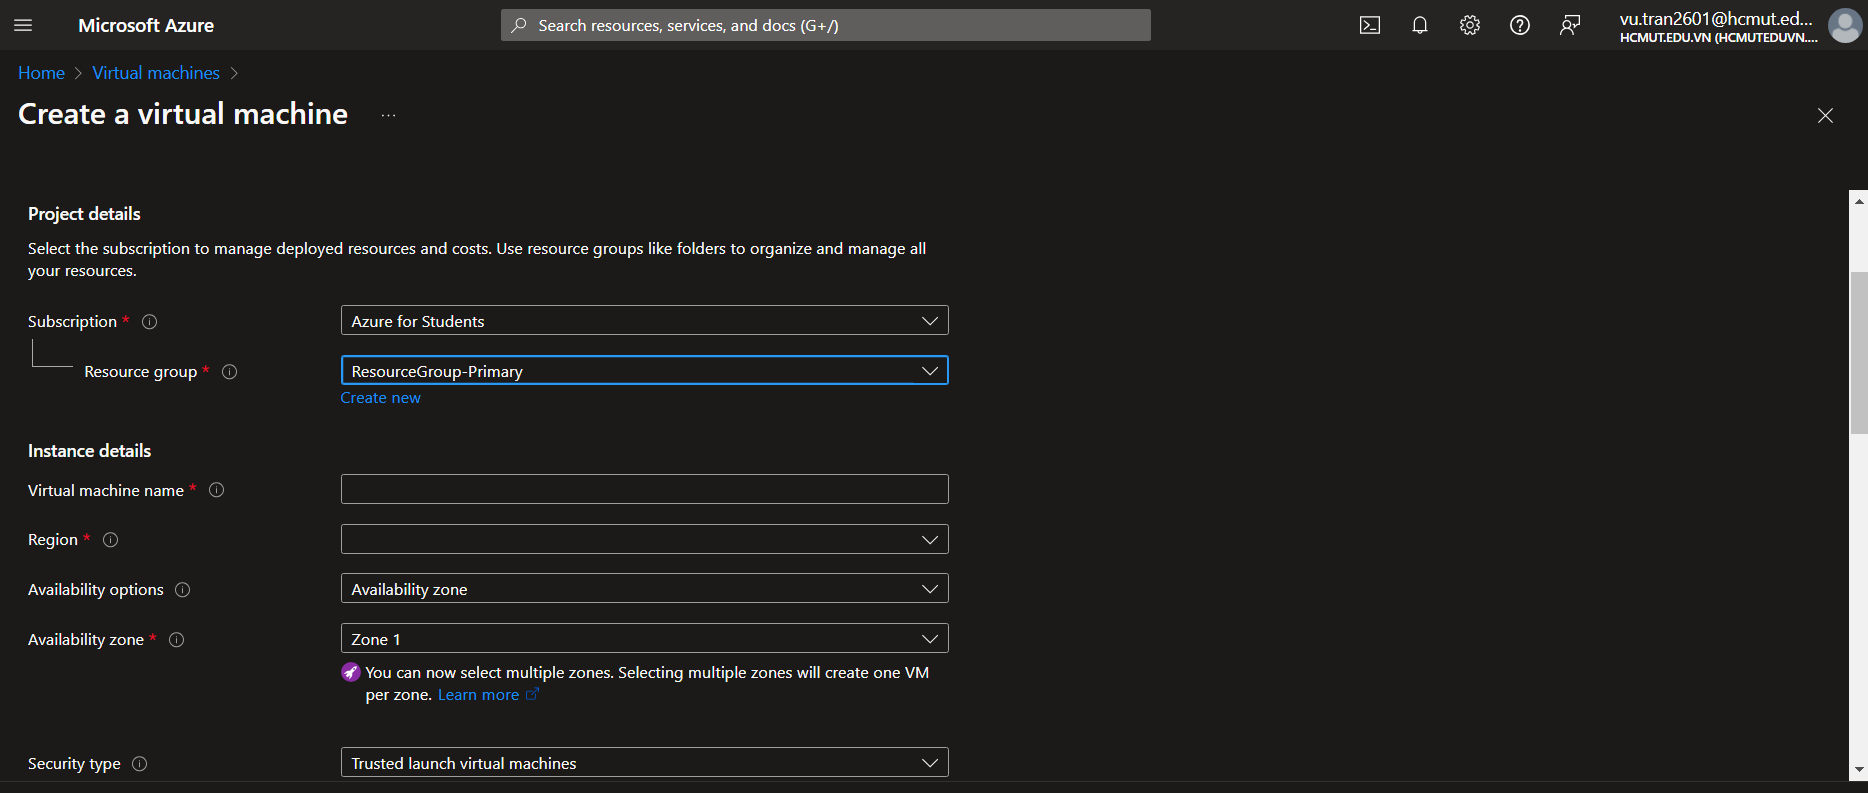
\includegraphics[width=1\textwidth]{Images/Deployment/HybridSearch/Config1.png}
    \caption{Thiết lập cấu hình cho máy ảo Azure VM}
\end{figure}
\begin{figure}[H]
    \centering
    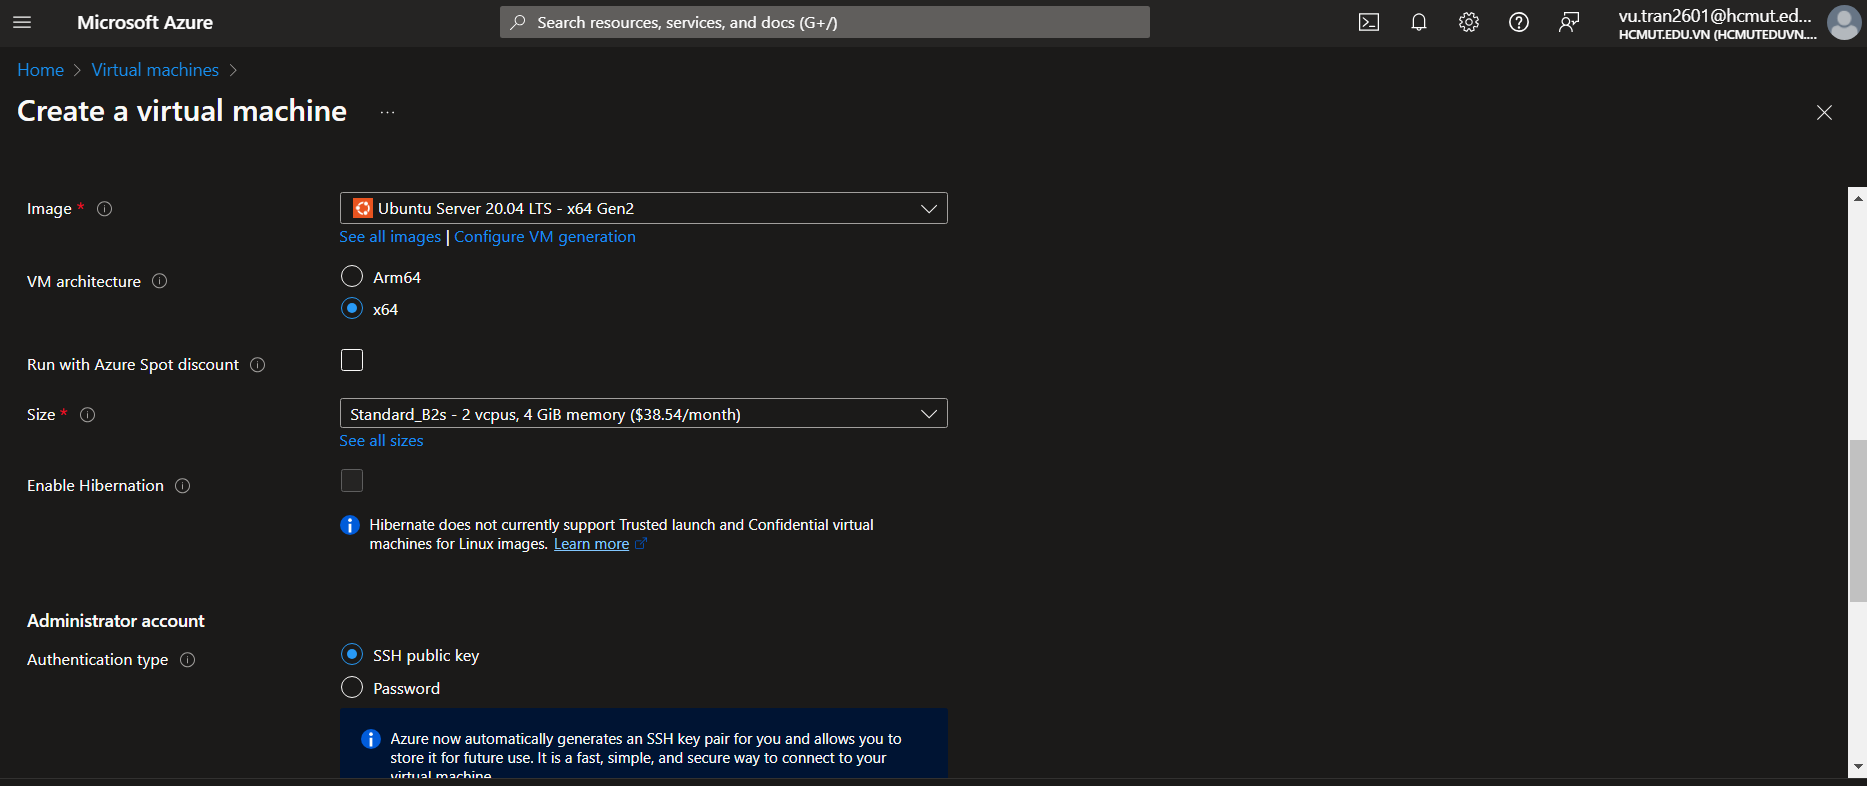
\includegraphics[width=1\textwidth]{Images/Deployment/HybridSearch/Config2.png}
    \caption{Thiết lập cấu hình cho máy ảo Azure VM}
\end{figure}
\begin{figure}[H]
    \centering
    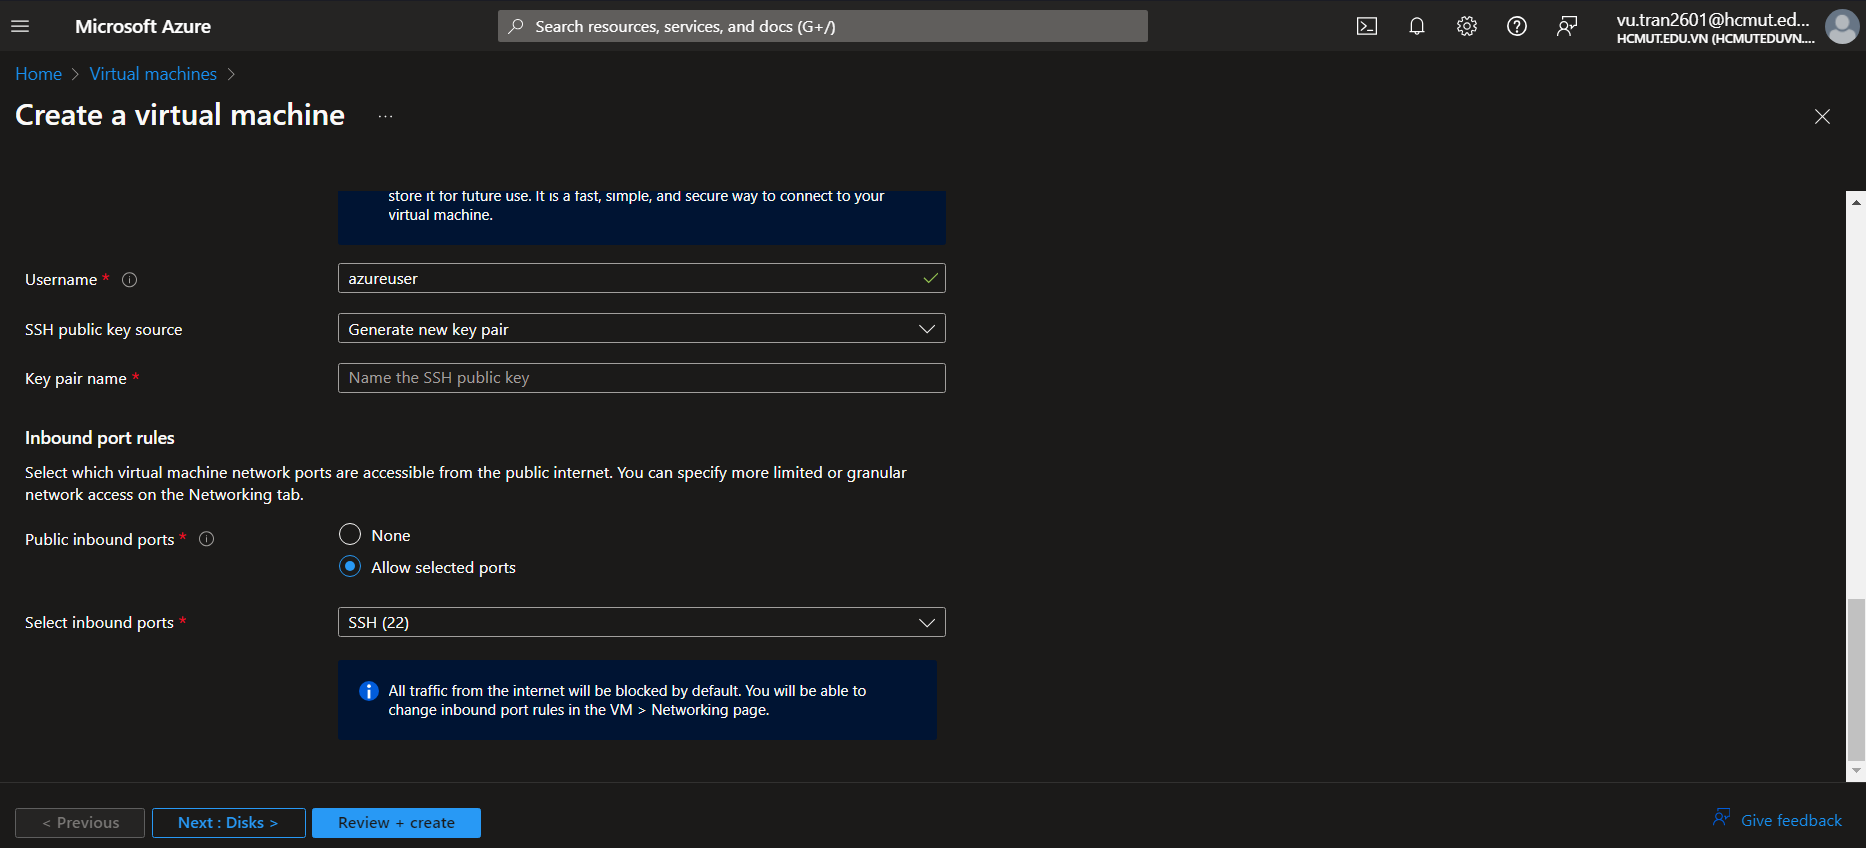
\includegraphics[width=1\textwidth]{Images/Deployment/HybridSearch/Config3.png}
    \caption{Thiết lập cấu hình cho máy ảo Azure VM}
\end{figure}
\hspace*{1cm}
Các bước thiết lập cấu hình máy ảo \textit{Azure VM} có phần hơi phức tạp, cụ thể các bước cấu hình như sau:
\begin{itemize}
    \item \textit{Subscription:} Ở mục này, ta cần chọn gói thuê bao để \textit{Azure} sẽ thực hiện tính phí cho dịch vụ máy ảo. Ở đây, do nhóm đã đăng ký tài khoản học sinh, sinh viên nên sẽ chọn \textit{Azure for Students}.
    \item \textit{Resource Group:} Ở mục này, ta cần chọn nhóm tài nguyên mà ta đã tạo sẵn ở bước trên, trong mục này, nhóm sẽ chọn \textit{ResourceGroup-Primary}.
    \item \textit{Virtual machine name}: Ở mục này, ta cần đặt tên cho máy ảo.
    \item \textit{Region:} Ở mục này, ta cần lựa chọn vị trí máy chủ nơi mà dịch vụ máy ảo sẽ được triển khai, trong mục này nhóm sẽ chọn \textit{(Asia Pacific) Southeast Asia}, vì vị trí này gần với Việt Nam nhất.
    \item \textit{Availability options:} Ở mục này, ta có thể để giữ nguyên lựa chọn mặc định là \textit{Avaiability zone}
    \item \textit{Availability zone:} Ở mục này, ta cần chọn các \textit{zone} để triển khai máy ảo, mặc định sẽ chọn triển khai ở \textit{Zone 1}, ta có thể giữ nguyên mục này.
    \item \textit{Security type:} Ở mục này, mặc định sẽ là \textit{Trusted launch virtual machines}. Các lựa chọn khác nhau ở mục này sẽ xác định mức độ bảo vệ cho máy ảo.
    \item \textit{Image:} Ở mục này, ta cần chọn hệ điều hành cho máy ảo, ở đây nhóm sẽ chọn hệ điều hành \textit{Ubuntu Server 22.04 LTS - x64 Gen2} để triển khai máy ảo.
    \item \textit{VM architecture:} Ở mục này, ta sẽ chọn kiến trúc vi xử lý của máy ảo, mặc định lựa chọn ở mục này sẽ là kiến trúc \textit{x64}.
    \item \textit{Size:} Đây là mục quan trọng, ta cần chọn kích thước cho phần cứng của máy ảo, phần này sẽ quyết định đến giá tiền sử dụng dịch vụ, để đảm bảo khả năng vận hành của mô hình \textit{hybrid search}, cũng như để tiết kiệm chi phí một cách tối ưu, nhóm đã chọn kích thước \textit{Standard\_B2s - 2 vcpus, 4GiB memory}, với giá mà \textit{Azure} ước tính sẽ rơi vào khoảng \$38.54 cho một tháng.
    \item \textit{Authentication type:} Ở mục này, ta cần chọn phương thức xác thực để kết nối đến máy ảo, ở đây nhóm chọn xác thực bằng \textit{SSH}.
    \item \textit{Username:} Ở đây ta cần đặt một tên tài khoản cho bước xác thực khi đến nối đến máy ảo \textit{Azure}.
    \item \textit{SSH pblic key source:} Để thuận tiện hơn, ở mục này ta chọn \textit{Generate new key pair} và đặt tên cho \textit{public key}.
    \item \textit{Public inbound ports:} Ở đây để có thể kết nối đến máy ảo từ \textit{internet}, ta có thể chọn \textit{Allow selected ports} và tương ứng với mục phía dưới \textit{Select inbound ports}, ta có thể để mặc định là \textit{SSH(22)}. Như vậy, máy ảo sẽ có thể được kết nối từ bất kì đâu và sẽ chấp nhận kết nối bằng giao thức \textit{SSH} ở cổng \textit{22}.
\end{itemize}
\hspace*{1cm}
Đến đây, ta có thể chọn \textit{Review + create} để kiểm tra lại một lần nữa tất cả các cài đặt và cấu hình cho máy ảo, sau khi đã hoàn tất. Ta có thể nhấn vào \textit{Create}, và lúc này vì đã chọn ở bước phía trên là \textit{Generate new key pair}, nên trang chủ sẽ hiện một \textit{pop-up} để đề nghị tải xuống \textit{private key} cho bước xác thực \textit{SSH}. Ở bước này, ta cần tải về và lưu trữ \textit{private key} ở một nơi an toàn trên máy tính. Sau khi đã tải về, ta cần cấp quyền \textit{Full control} cho người dùng của hệ điều hành để tránh bị báo lỗi khi thực hiện kết nối với máy ảo.
\begin{figure}[H]
    \centering
    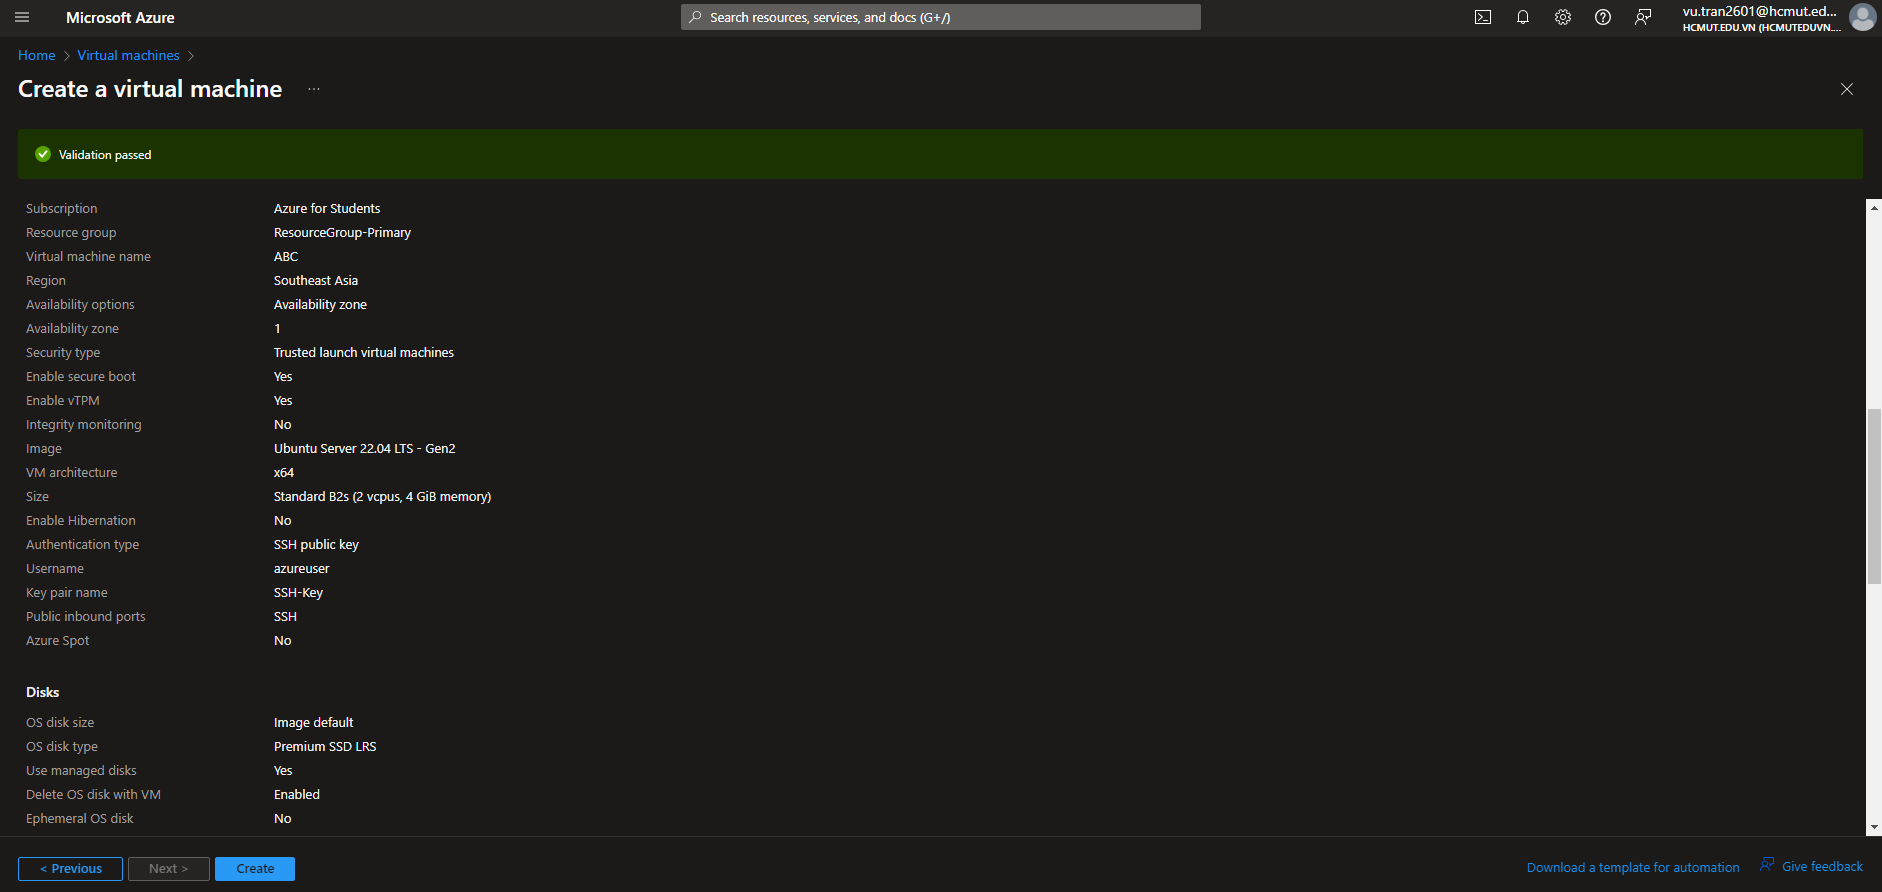
\includegraphics[width=1\textwidth]{Images/Deployment/HybridSearch/ReviewCreate.png}
    \caption{Kiểm tra lại các cài đặt trước khi tạo máy ảo Azure VM}
\end{figure}
\begin{figure}[H]
    \centering
    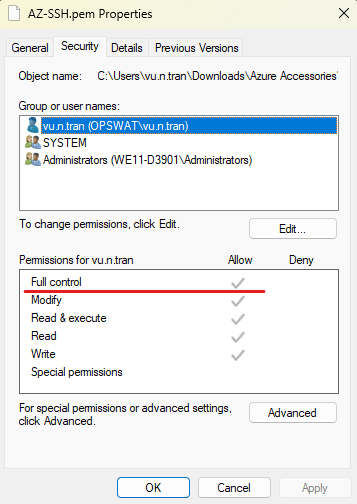
\includegraphics[width=0.5\textwidth]{Images/Deployment/HybridSearch/FullControl.png}
    \caption{Cấp quyền full control cho SSH private key}
\end{figure}
\hspace*{1cm}
Đến đây ta có thể kết nối đến máy ảo bằng \textit{command line}, ta có thể sử dụng \textit{Windows Powershell} để kết nối đến địa chỉ \textit{IP} của máy ảo với tên đăng nhập và \textit{SSH private key} mà ta đã khởi tạo ở bước trên.
\begin{figure}[H]
    \centering
    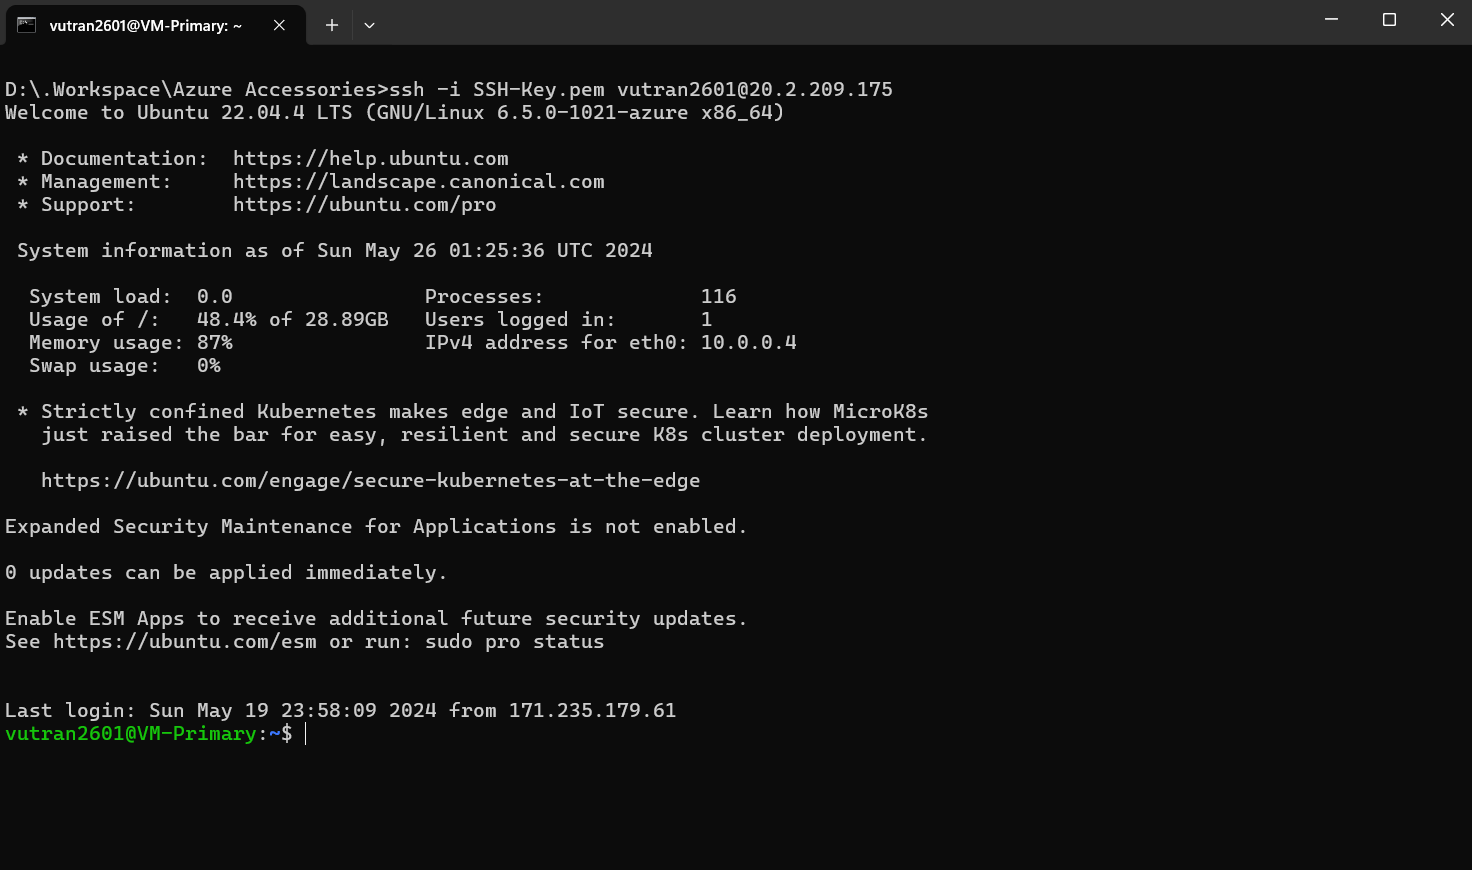
\includegraphics[width=1\textwidth]{Images/Deployment/HybridSearch/VM-Connection.png}
    \caption{Khởi tạo kết nối đến máy ảo Azure VM}
\end{figure}
\hspace*{1cm}
Tiếp theo, ta cần phải chạy được ứng dụng trên máy ảo \textit{Azure VM} tương tự như cách ta chạy ở \textit{localhost}. Tuy nhiên, vì ta cần cho phép các kết nối công khai đến ứng dụng \textit{Flask} đang triển khai ở máy ảo này. Có nhiều phương pháp để thực hiện mục tiêu trên, tuy nhiên để cho đơn giản và nhanh chóng, nhóm sử dụng công cụ \textit{ngrok}, \textit{ngrok} là một công cụ phần mềm cho phép người dùng tạo các đường hầm bảo mật từ một mạng công cộng đến một máy tính hoặc thiết bị cụ thể trong mạng cục bộ của người dùng. Công cụ này thường được sử dụng để:
\begin{itemize}
    \item Triển khai và thử nghiệm ứng dụng \textit{web} cục bộ: Ngrok tạo ra một \textit{URL} công cộng (dạng \url{https://<subdomain>.ngrok.io}) cho phép người dùng truy cập trực tiếp vào ứng dụng web chạy trên máy tính cá nhân của người dùng từ bất kỳ đâu trên \textit{internet}.
    \item Phát triển \textit{webhook}: Khi phát triển các dịch vụ \textit{webhook}, như nhận thông báo từ \textit{Stripe}, \textit{GitHub}, hoặc \textit{Slack}, người dùng có thể sử dụng \textit{ngrok} để nhanh chóng nhận và thử nghiệm các yêu cầu \textit{HTTP} từ các dịch vụ này đến máy chủ cục bộ của người dùng.
    \item Chia sẻ dự án nhanh chóng: Người dùng có thể chia sẻ phiên bản đang phát triển của một trang \textit{web} hoặc ứng dụng với đồng nghiệp hoặc khách hàng mà không cần phải triển khai lên một máy chủ công cộng.
\end{itemize}
\hspace*{1cm}
\textit{Ngrok} hoạt động bằng cách chạy một ứng dụng máy khách trên máy tính của người dùng. Ứng dụng này kết nối với các máy chủ của \textit{ngrok} thông qua một kết nối bảo mật. Khi người dùng khởi chạy \textit{ngrok}, nó sẽ tạo ra một \textit{URL} công cộng và chuyển tiếp tất cả các yêu cầu tới \textit{URL} đó đến máy tính cục bộ của người dùng thông qua kết nối bảo mật.\\
\hspace*{1cm}
Để thiết lập \textit{ngrok} trên máy ảo \textit{Azure VM}, ta cần phải có tài khoản \textit{ngrok}, sau đó truy cập vào trang \textit{web} của \textit{ngrok} để lấy mã \textit{token} ứng với tài khoản đang sử dụng. Và sau đó, ở giao diện \textit{command line} của máy ảo \textit{Azure VM}, ta cần chạy câu lệnh:
\begin{lstlisting}
ngrok config add-authtoken <token>
\end{lstlisting}
\hspace*{1cm}
Bước tiếp theo, ta cần thiết lập \textit{ngrok} ở trong mã nguồn của mô hình tìm kiếm \textit{hybrid}, ở bước này, ta cần thêm các dòng sau trong \textit{file app.py}, để mỗi khi ứng dụng \textit{Flask} khởi chạy, ứng dụng sẽ tạo ra một \textit{URL} công khai để bất kì thiết bị nào cũng có thể kết nối đến ứng dụng:
\begin{python}
from pyngrok import ngrok

# Open a ngrok tunnel to the HTTP server
public_url = ngrok.connect(5000).public_url
print(' * ngrok tunnel "{}" -> "http://127.0.0.1:{}/"'.format(public_url, 5000))

# Update any base URLs to use the public ngrok URL
app.config["BASE_URL"] = public_url
\end{python}
\hspace*{1cm}
Cuối cùng, ta cần \textit{commit} và \textit{push} mã nguồn lên \textit{GitHub}, sau đó ta chuyển qua giao diện \textit{command line} của máy ảo \textit{Azure VM} để \textit{clone} mã nguồn về, ở bước này ta cần phải có \textit{Personal access token} của \textit{GitHub}, để lấy được \textit{access token} này, ta cần vào bên trong cài đặt tài khoản cá nhân của \textit{GitHub} để sử dụng. Sau khi ta đã \textit{clone} được mã nguồn thành công, bước tiếp theo ta cần cài đặt các \textit{package} kèm theo của ứng dụng. Sau đó ta cần sử dụng lệnh \textit{tmux} để tạo ra một \textit{command line session} riêng trên máy ảo, ta cần phải làm như vậy để khi ngắt kết nối khỏi máy ảo thì \textit{command line} vẫn tiếp tục chạy như bình thường, và do đó sẽ giúp cho ứng dụng không bị ngưng khi ta thoát khỏi máy ảo. Và cuối cùng, ta chỉ cần chạy câu lệnh \textit{flask run} để khởi động ứng dụng mô hình tìm kiếm \textit{hybrid}. Khi ứng dụng được khởi chạy, giao diện \textit{command line} hiển thị địa chỉ \textit{URL} để truy cập đến ứng dụng, ta cần lưu giữ địa chỉ \textit{URL} này để kết nối về sau. Để thoát ra khỏi \textit{command line} đang chạy ứng dụng, ta cần nhấn tổ hợp phím \textit{Ctrl + B}, sau đó nhấn phím \textit{D}. Như vậy, ta có thể tạm thời ngắt kết nối đến \textit{command line} mà vẫn giữ cho ứng dụng tiếp tục được hoạt động mà không bị dừng. Đến đây, ta đã hoàn thành việc triển khai ứng dụng mô hình tìm kiếm \textit{hybrid} trên máy ảo \textit{Azure VM}